\documentclass[a4paper,10pt]{article}

\usepackage{fancyhdr}
\usepackage{graphicx}
\usepackage{geometry}
\geometry{a4paper, left=2cm, right=2cm, top=1.5cm, bottom=4cm }
\usepackage{caption}
\usepackage{subcaption}
\usepackage{hyperref}
\usepackage[square,numbers]{natbib}
%\usepackage{cite}





\usepackage{etoolbox,fancyhdr,xcolor}
\newcommand{\headrulecolor}[1]{\patchcmd{\headrule}{\hrule}{\color{#1}\hrule}{}{}}
\newcommand{\footrulecolor}[1]{\patchcmd{\footrule}{\hrule}{\color{#1}\hrule}{}{}}
\renewcommand{\headrulewidth}{1pt}
%\headrulecolor{black!100}%
\renewcommand{\footrulewidth}{1pt}
\footrulecolor{black!100}%

\fancyhf{}
\fancyhead[R]{\includegraphics[width=0.25\textwidth]{figures/fjfi.png}}

\fancyfoot[L]{Project: Jets}
\fancyfoot[C]{Faculty of Nuclear Sciences and Physical Engineering, CTU}
\fancyfoot[R]{\thepage}

\setlength{\headheight}{26mm}
\pagestyle{fancy}

%\bibliographystyle{IEEEtran}
%\bibliography{ResearchPaperBib}{}


\usepackage{times}
\begin{document}

\noindent 
\begin{center}
\textbf{{\Large JETS IN PP AT THE LHC}} \\
\end{center}

\vskip1cm
\noindent 
\textbf{Author: Bc. M Vranovský,} \textit{Czech Technical University in Prague}
\\

%\noindent %supervisor
%\textbf{Research Supervisor: D. Duck,} \textit{University of Bristol, Bristol, U.K.}


\section*{INTRODUCTION}
This is a report on a project with topic Jets in \textit{pp} collisions at the Large Hadron Collider (LHC), moreover at the LHC energies of collision. The goal of the project is to generate events with a Monte Carlo generator, analyze them with focus on jets and jet finding. In the end, discuss results and compare them to existing data. In \autoref{jets}, jets will be introduced and discussed. Following, will be \autoref{soft}, where all the software used and the written code is discussed. The entire code in C++ used for the analysis of generated events can be found on GitHub\cite{GitHubJets}. Lastly, in \autoref{results} results are shown and discussed. Results are also compared to measurements from experiments at the LHC and at the Relativistic Heavy Ion Collider (RHIC).

\section{JETS}
\label{jets}
Large accelerators and colliders such as the Large Hadron Collider (LHC) in CERN or the Relativistic Heavy Ion Collider (RHIC) are designed to study the strong force at very high temperatures when quarks and gluons are melted into something that is called the Quark Gluon Plasma (QGP)\cite{Cunqueiro_2022}. QGP is a state of matter in which quarks are not bound to each other by gluons, but are moving almost freely. One of the first times the QGP has been mentioned, was by Rolf Hagedorn in his article "Statistical thermodynamics of the strong interaction"\cite{hagedorn} when he referred to them as small fireballs. These small fireballs are created in high energy heavy ion collisions for only a brief moment. One of ways these fireballs are studied is through something called jets. Jets are created at the beginning of a high energy collision by transferring large portion of transverse momentum to a single or more strongly interacting particles. 
\newline
\noindent A jet can be understood as a collimated\footnote{By collimated one means that all particles that are part of the jet have similar azimuthal angle and rapidity.} shower or spray of hadrons detected by a detector or a system of detectors. All the particles which are part of a jet come from a single particle in the beginning- a quark or a gluon. This initial particle is ejected from a color neutral state with high transverse momentum. As it is flying towards a detector with high energy, it produces gluonstrahlung\footnote{Gluonstrahlung is similar to bremstrahlung in classical physics, when a highly energetic particle emits photons in the direction of it's momentum with which it loses energy.\cite{L2016Radioactivity}} and decays to more stable states. Very often jets are produced in pairs called dijets which is mostly because of conservation of momentum. The created jets are flying in the opposite directions from the point of interaction. 
\newline
\noindent Because jets are created in the beginning of a collision, they hold information about the entire process. One is able to use them as a probe to gain and extract information and evidence about the QGP. An argument for the existence of QGP is a process called jet quenching. This occurs in heavy-ion collisions when a dijet is created close to the surface. The detector should be measuring 2 jets on the opposite sides of the detector, but only measures one. That is because one of the jets has to traverse the Quark Gluon Plasma where it interacts with many other particles and loses energy via secondary interactions. This phenomenon is not observed in \textit{pp} collisions because QGP is not created there and therefore both jets can be seen\cite{casalderreysolana2007introductory}.


\section{SOFTWARE}
\label{soft}
This section discusses the software used for analysis. First, events where generated by Pythia 8, which is described in \autoref{pyth}, then jets where reconstructed with algorithm provided by FastJet3 described in \autoref{fas}. Lastly, the analysis code is briefly described in \autoref{code}.

\subsection{Pythia 8}
\label{pyth}
Pythia\cite{PythiaPythia} is an open-source Monte Carlo generator of high energy collisions. It is designed to be a general purpose generator, therefore it is widely used in many analyses. It is written in C++ programming language as most of infrastructure at large experiments around the world. The generator includes theory, models and perturbative calculations often even to NLO\footnote{NLO stands for Next to Leading Order in perturbative calculations.} to describe as many processes with the highest accuracy\cite{pythiaSjostrand}. Calculations used to generate events are regularly updated based on new physical measurements and results. Pythia can also be used as a baseline generator and can be modified by users to describe better some specific processes. 
\newline
\noindent In language of high energy physics, an event is considered an interaction between 2 particles that are being collided together. Because particle physics includes very high number of different processes with infinitely many possible outcomes, an event generator is based on randomness as well as previous measurements, which show that some specific processes are more probable than others\cite{Pythia2022comprehensive}. Even the number of outgoing particles can vary: from a few particles to events with thousands of produced particles. It is necessary to mention, that event generators are only based on the current understanding of laws of nature and are not the laws themselves. Therefore, it is crucial for physicists to always be comparing the actual measured data to results from event generators to point out the differences between the two and try to understand them.
\newline
\noindent The evolution of an event generated by Pythia is best described at 3 different stages. The first is the \textit{ProcessLevel} which administrates the choice of process based on a combination of matrix element expressions and phase space selection\cite{pythiaSjostrand}. The next stage is the \textit{PartonLevel}, when the process looks more closely at smaller scales, multiple interactions between particles. The last stage is the \textit{HadronLevel} when partons undergo process of hadronization and produce particles that are usually detected by one of subsystems of a large detecting system.


\subsection{Jet algorithms and FastJet}
\label{fas}
In \autoref{jets}, jets have been briefly introduced, but not defined properly. A collimated shower of hadrons is a vague definition, especially in the field of HEP. For jet classification and categorization one uses jet finding algorithms.  Jet finding algorithms are based on 2 different methods.
\newline
\noindent  The first one is the cone algorithm when one defines a cone with some specific radius which begins at the point of interaction and ends at the surface of the detector. Particles that are in the cone belong to the jet. The problem with this algorithm is the initial definition of radius of the cone. Some jets are very narrow and having a wide radius would mean pile-up from particles that do not belong to the jet. On the other hand, some jets can be wider than the lines of the cone and therefore not all particles would be included in the jet\cite{Catani:2000xqw}. 
\newline
\noindent The second method is called sequential recombination\cite{Tseng_2013}. This algorithm is so-called bottom-up when one looks at the 2 closest particles, recombines them and then continues the recombination process with the closest particle to this pair and so on. The recombination process is based on minimizing distances between final state particles\cite{Tseng_2013}. In the end, the 4-momenta of all particles involved in a jet are summed from which one gets the energy of the entire jet. Some of sequential recombination algorithms are $k_t$, anti-$k_t$ or Cambridge/Aachen.
\newline
\noindent FastJet is a C++ software, which implements the most used algorithms. FastJet is user friendly and the implementation can be described in only a few steps. First of all, one defines the type of algorithm which is going to be used. That is done using the implemented JetDefinition class. In addition, one also defines there radius R, which is part of minimizing process in sequential recombination\cite{FastJet2011FastJet}. Then, one uses PseudoJet class to enter all particles from which the clustering algorithm will create jets. PseudoJet class needs the 4-momentum of a particle and can play the role of a single particle as well as multiple particles that make up a jet. The entire clustering is done using class ClusterSequence. In the end, one can sort the jets using function \textit{sorted\_by\_pt()}. To reduce the overall number of jets in an event, one often uses a minimum transverse momentum condition.

\subsection{Code description}
\label{code}
The entire code, as was mentioned before can be found on GitHub\cite{GitHubJets} with a README file with instructions on how to compile and run the code. The entire code is divided to 2 different parts based on the software that was used. The first part, called \textit{jetGenerator.cc}, uses Pythia to generate a number of events. At this point, it set to produce 100 events, but that can be changed easily. After every event is generated in function \textit{main()}, it is stored in a data structure TTree which is part of ROOT statistical framework developed by CERN for data analysis. A TTree is capable of storing multiple different events, where each event contains multiple tracks, and each track has it's properties stored in so-called branches\cite{CERN2018ROOT}. ROOT as all other software tools used in HEP, is written in C++. 
\newline
\noindent To be able to compare results to those measured in existing HEP detectors, only final state and charged particles are stored in TTree. This TTree is then stored in a TFile\footnote{Also data structure provided by ROOT. } under the name \textit{jetGen.root}. Very important part of the code is \textit{jetGenerator.cmnd}. It is a file, where one can change the settings for Pythia without having to recompile the program. Some of the settings used, are the energy of collision, the collided particles and the processes which are turned on in this analysis. The number of events that were generated is 100.
\newline
\noindent The second part of code in \textit{fastJetCluster.cc} is focused on reconstructing jets from the produced events. First, the TFile with data is loaded, TTree opened and then analyzed. The process of using FastJet was described in \autoref{fas}, here only the specific settings are discussed. Clustering was done using anti-$k_t$ algorithm with radius $R=0.4$. The minimum transverse momentum condition was set at $10$ GeV. After clustering was done, results were plotted again using ROOT. 

\section{RESULTS AND DISCUSSION}
\label{results}
This section discusses results and compares them measurements from colliders. First of all, it is important to mention that the number of events that were analyzed as part of this project was quite small and therefore the statistics is less significant. To compensate low statistics and to counteract bin migration, most histograms have wider binning. Nonetheless, some interesting phenomena can be recognized. 
\newline
\noindent Distribution of jets based on it's transverse before $p_T$ cut can be seen in \autoref{f1} and after in \autoref{f2}. One can see that the number of jets in interval from 0 to 10 GeV is much higher than for higher transverse momenta. The sequential recombination method which was used does not really look at the energy of a jet and only considers the distances between particles. That is why the condition on minimal transverse momentum is needed. From around 10 GeV the decrease is still visible, but is considerably less steep.

\begin{figure}[htbp]
    \centering
    \begin{minipage}{0.45\textwidth}
        \centering
        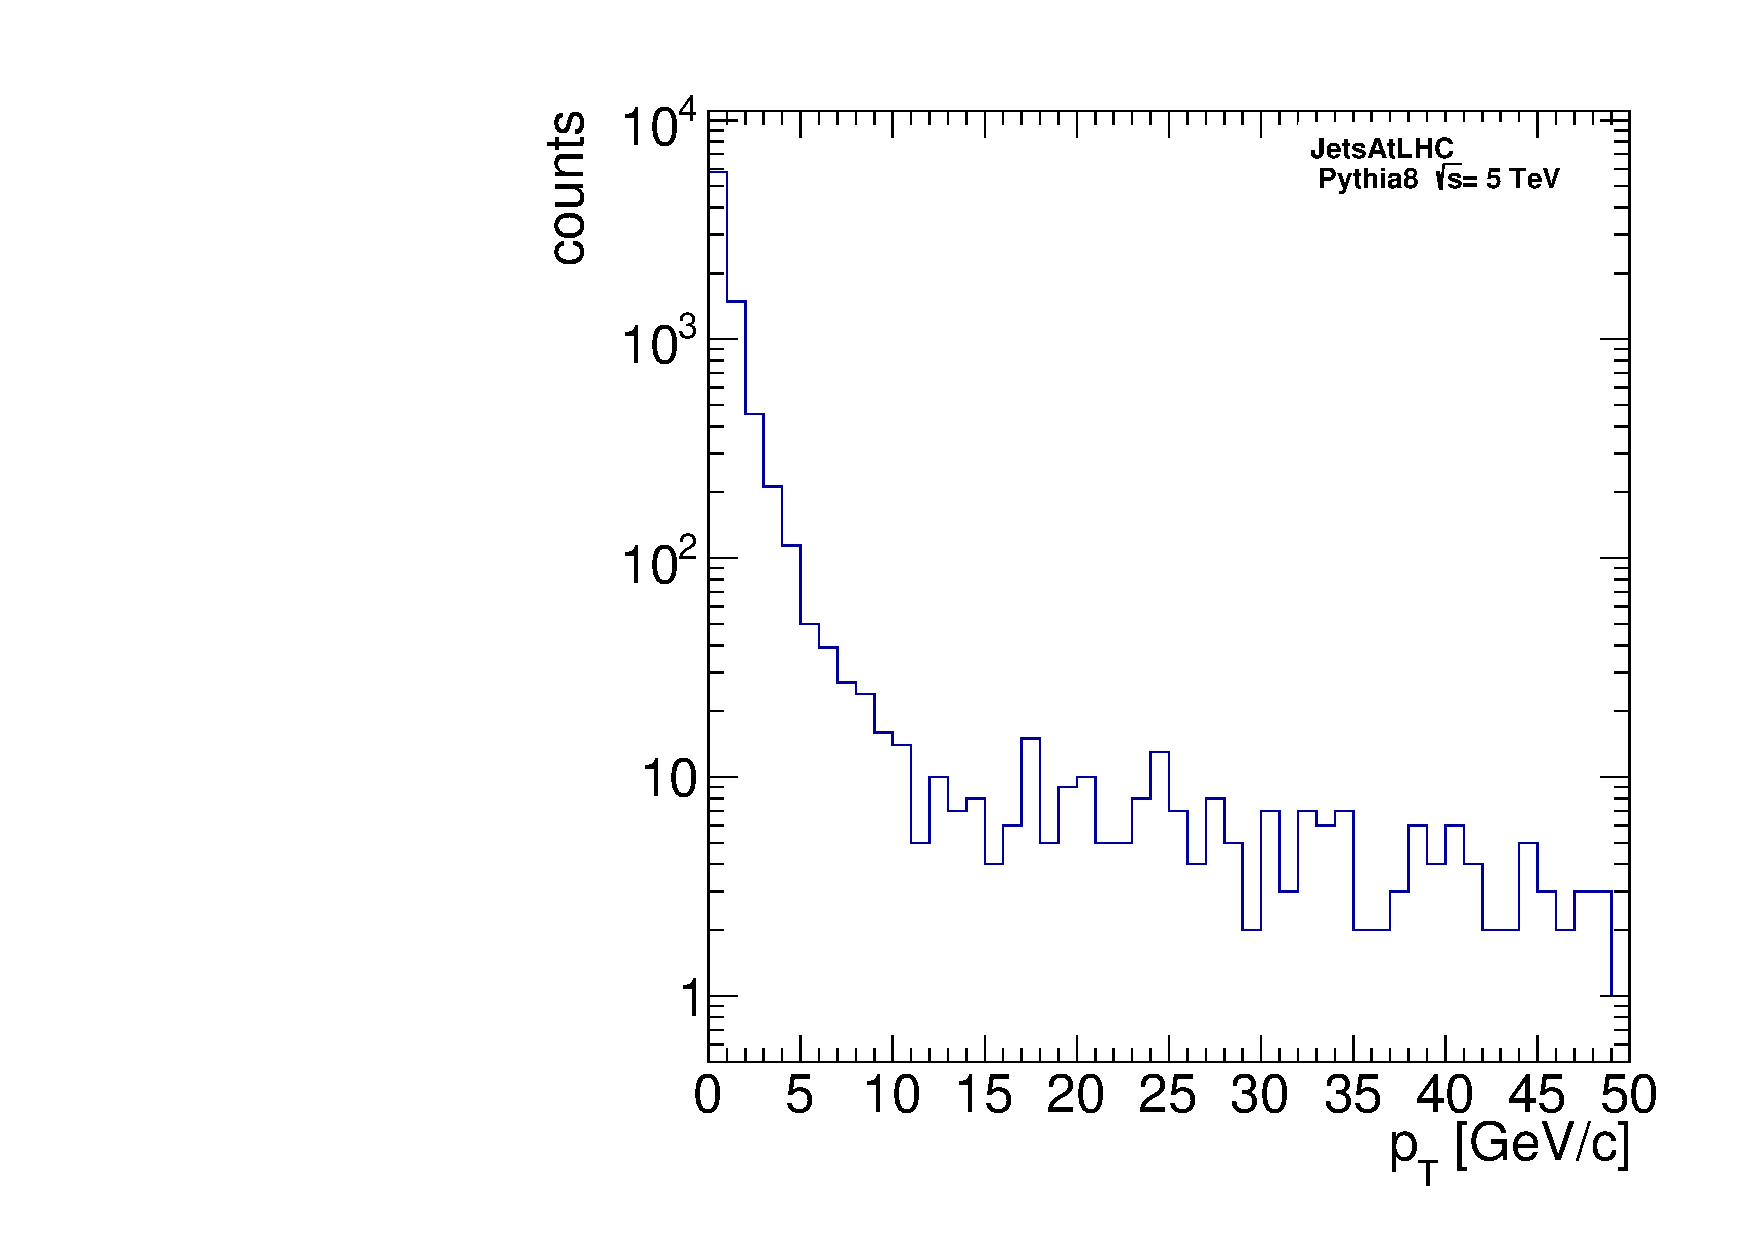
\includegraphics[width=\textwidth]{figures/hJetPt.pdf}
        \caption{Distribution of all jets recombined using sequential recombination method in all of 100 generated events. The \textit{y}-axis is logarithmic.}
        \label{f1}
    \end{minipage}\hfill
    \begin{minipage}{0.45\textwidth}
        \centering
        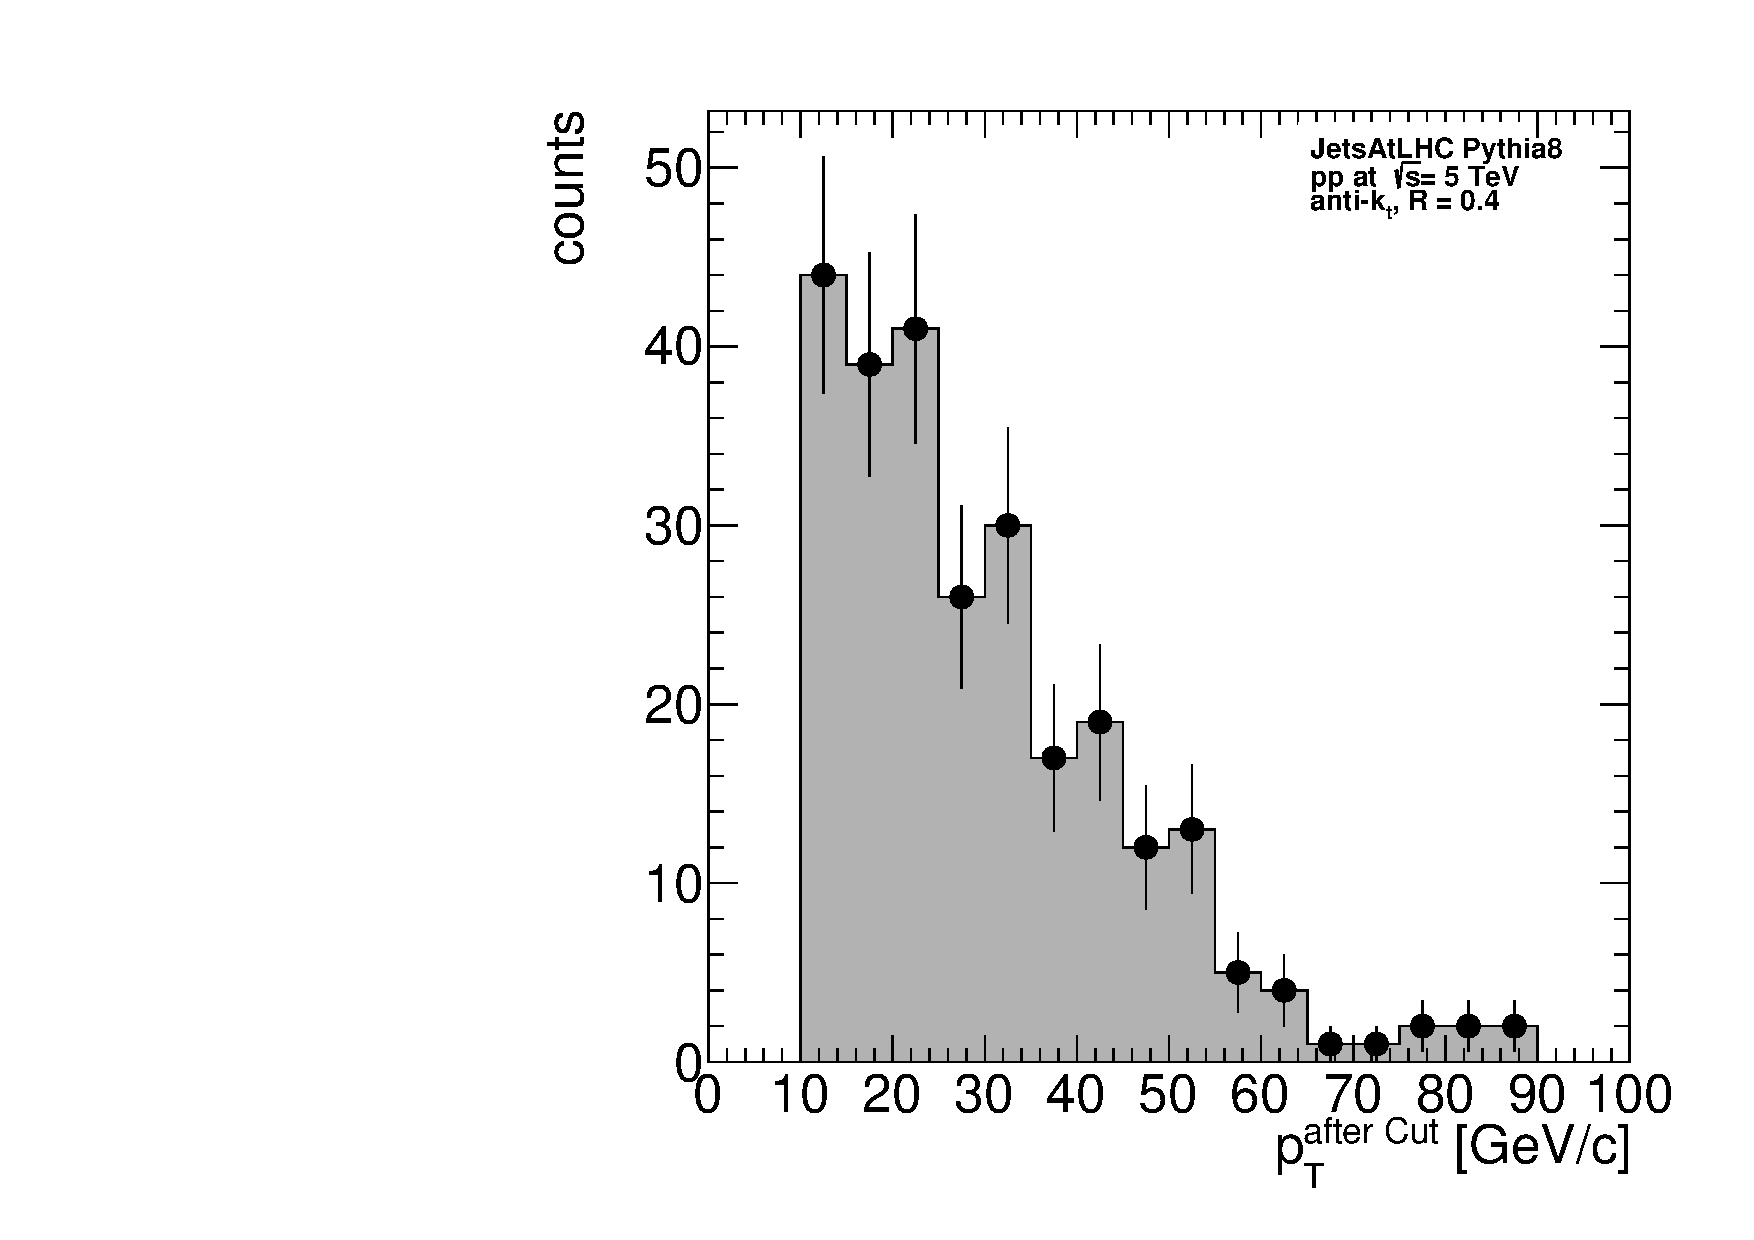
\includegraphics[width=\textwidth]{figures/hJetPtCut.pdf}
        \caption{Distribution of all recombined jets after cut on minimal transverse momentum. }
        \label{f2}
    \end{minipage}
\end{figure}

\noindent The importance of transverse momentum condition can be demonstrated also in the following plots. Histograms \autoref{f3} and \autoref{f4} show the number of jets per event before and after $p_T$ cut. Number of jets per event has rapidly decreased and therefore the background of less interesting events was suppressed. Distribution after the cut is centered around 3 jets per event. Another interesting distributions can be seen in \autoref{f5}. Figure shows the differences between rapidity \textit{y} and pseudorapidity $\eta$ distributions, where in this case both look almost identical. Because of the similarity, it is pointless to be showing results separately for y or $\eta$, especially in the next correlation plot. 
\newline
\noindent The demonstration of sequential recombination process, which takes place in the $(y,\phi)$ plane is shown in \autoref{f6}. It is a correlating distribution of all particles, while each jet is represented by a separate color and a marker. One can see that each jet is a cluster of particles- mostly hadrons collimated into a specific area. Differences between different jet clustering algorithms would be shown this type of plot.


\begin{figure}[htbp]
    \centering
    \begin{minipage}{0.45\textwidth}
        \centering
        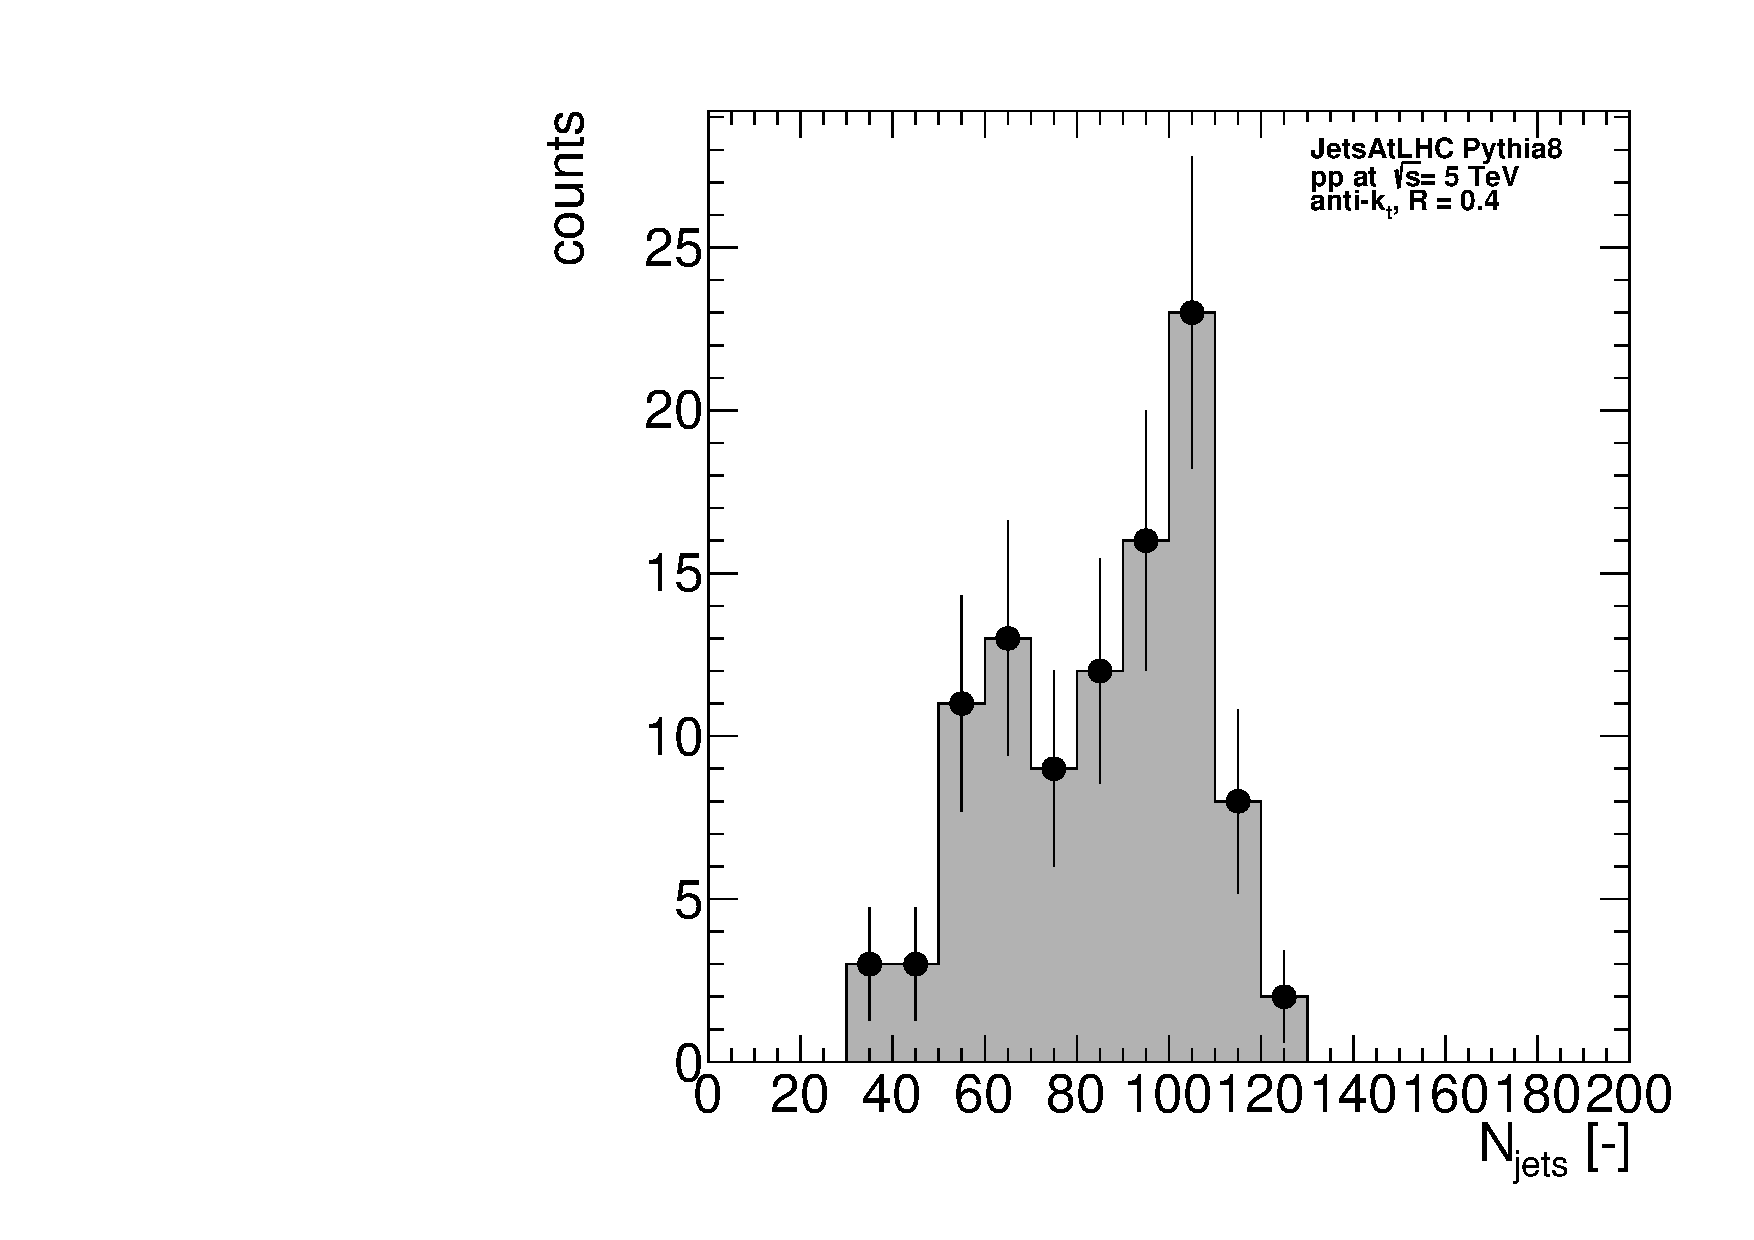
\includegraphics[width=\textwidth]{figures/hNJetsPerEvent.pdf}
        \caption{Distribution of number of jets per event before condition on transverse momentum.}
        \label{f3}
    \end{minipage}\hfill
    \begin{minipage}{0.45\textwidth}
        \centering
        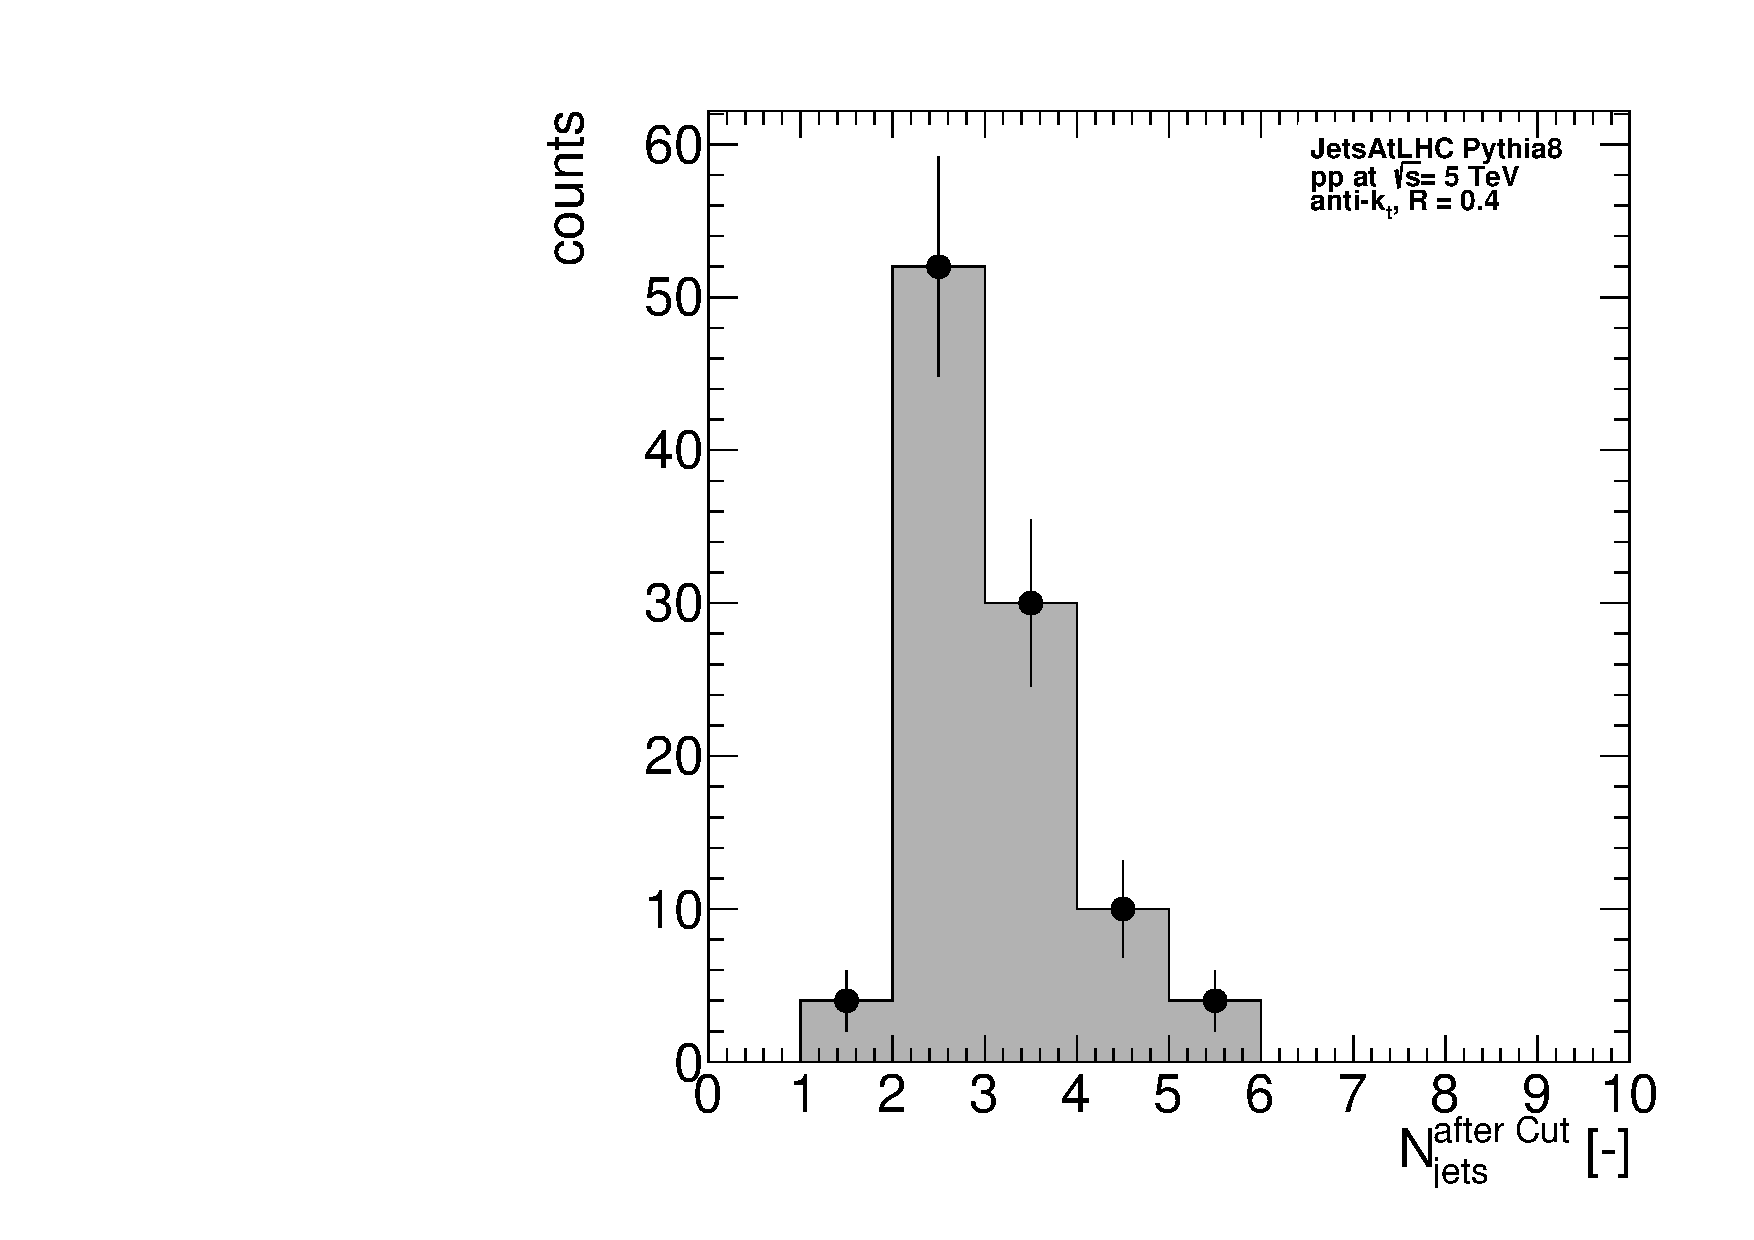
\includegraphics[width=\textwidth]{figures/hNJetsPerEventCut.pdf}
        \caption{Distribution of number of jets per event after transverse momentum condition. }
        \label{f4}
    \end{minipage}
\end{figure}


\begin{figure}[htbp]
    \centering
    \begin{minipage}{0.45\textwidth}
        \centering
        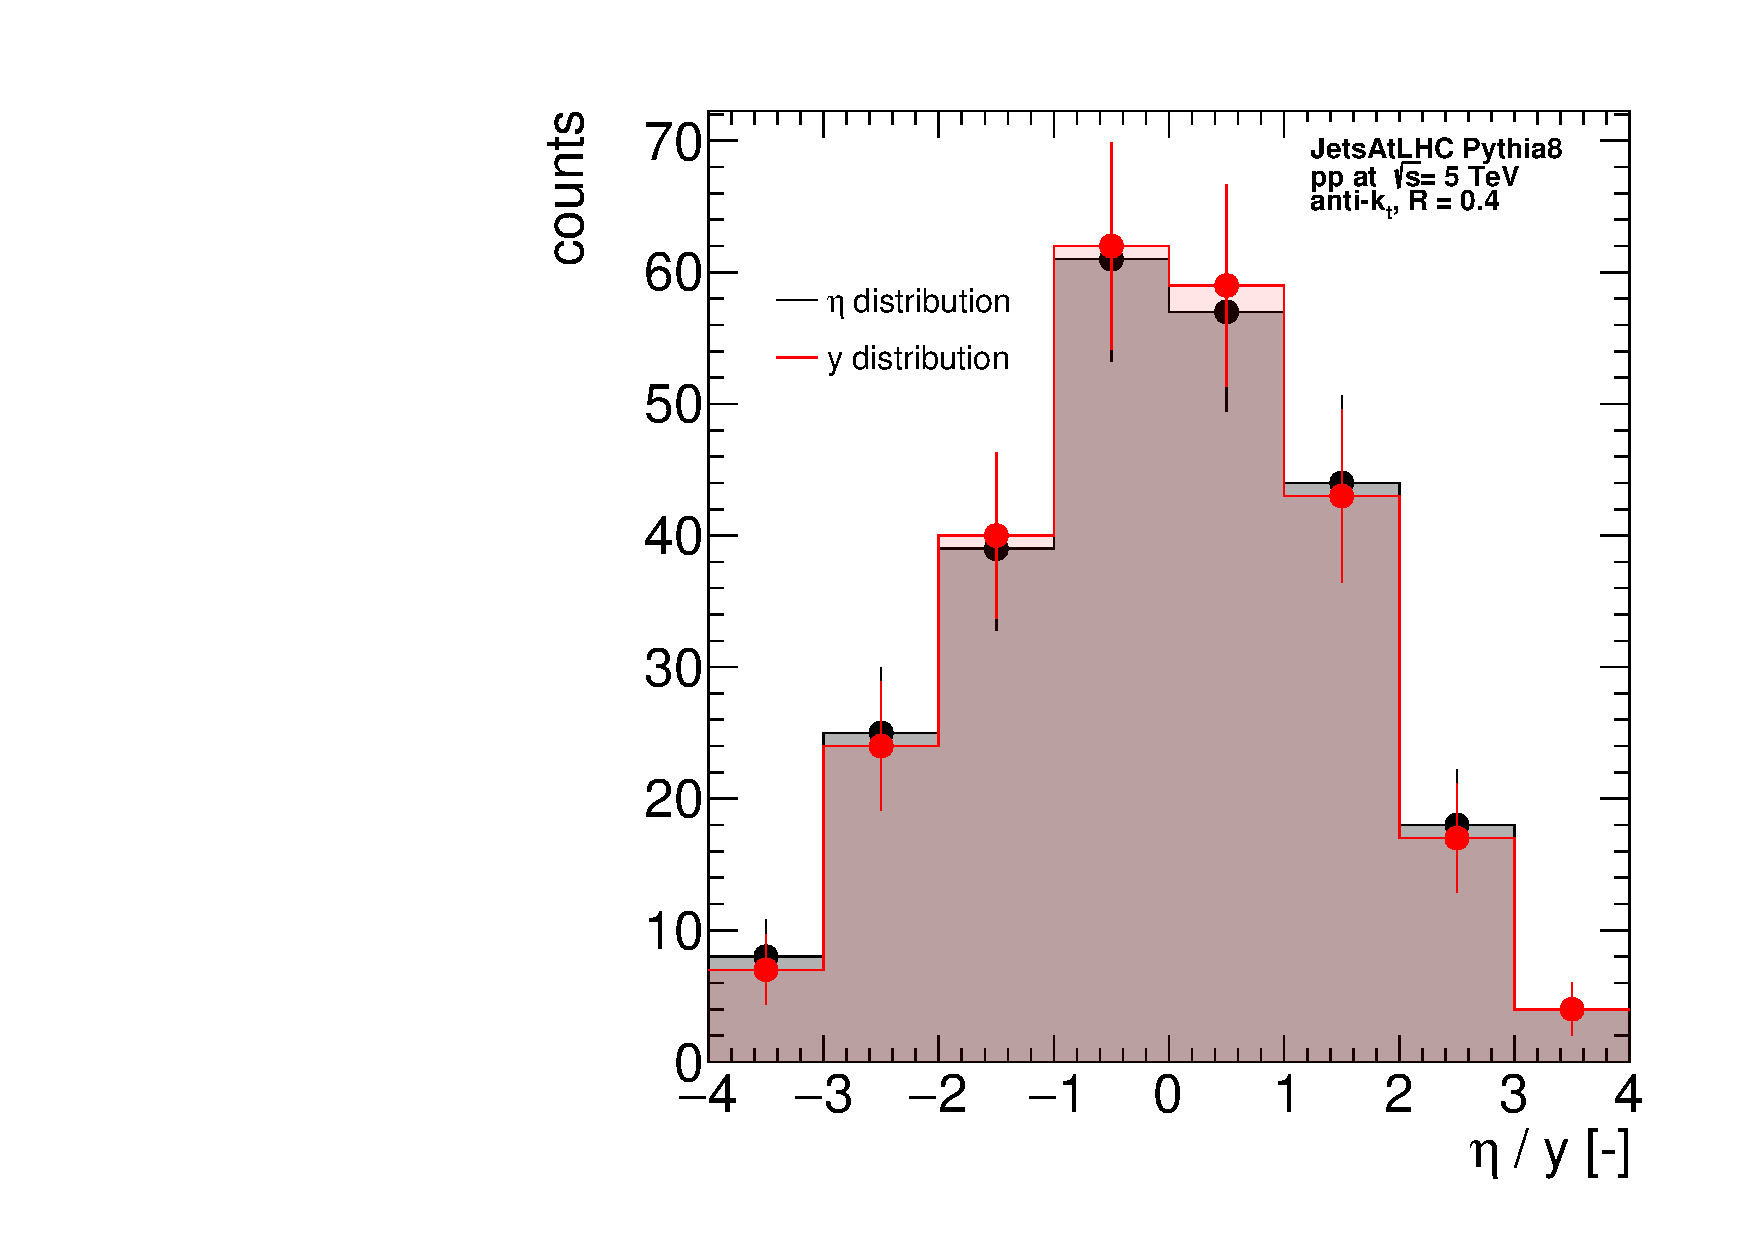
\includegraphics[width=\textwidth]{figures/hJetEta.pdf}
        \caption{Distribution of rapidity and pseudorapidity of jets that passed the transverse momentum condition. }
        \label{f5}
    \end{minipage}\hfill
    \begin{minipage}{0.45\textwidth}
        \centering
        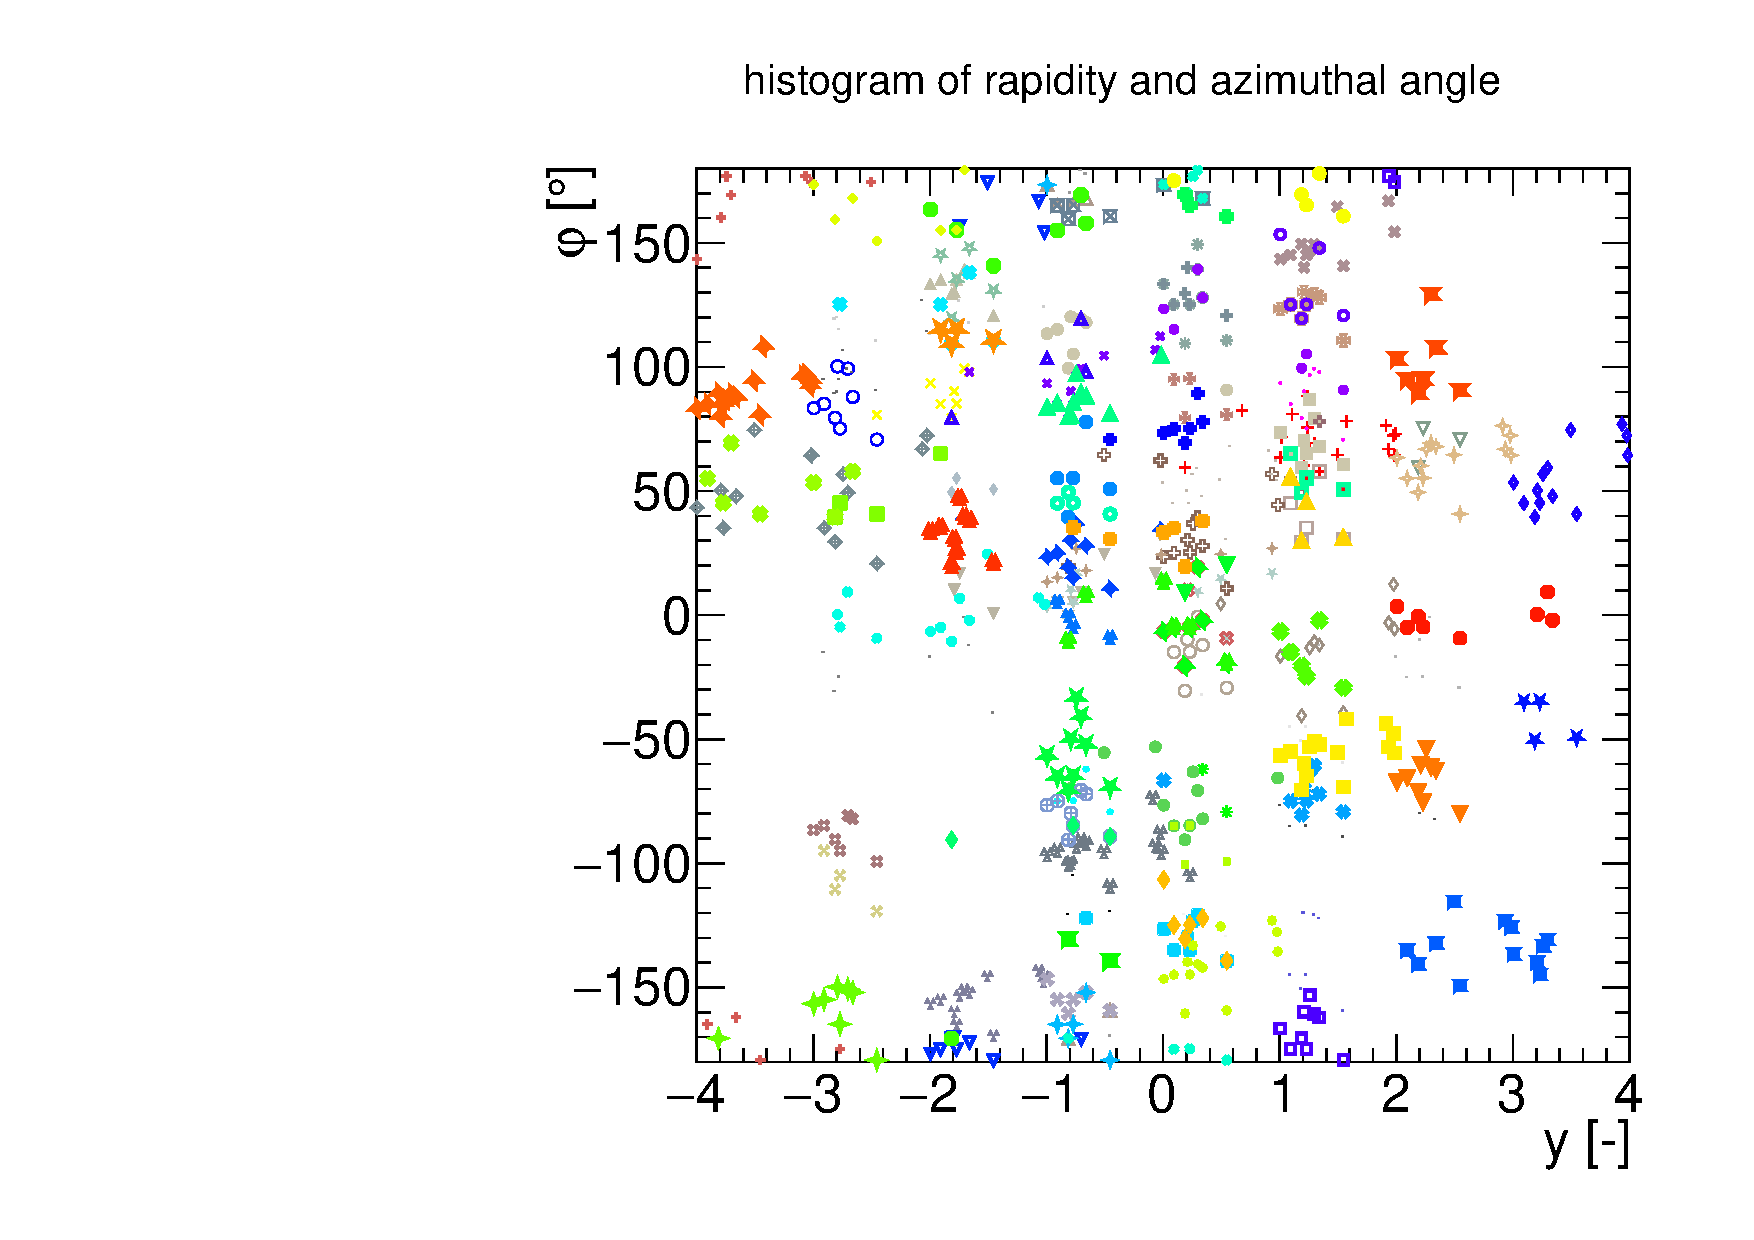
\includegraphics[width=\textwidth]{figures/hRapPhi.pdf}
        \caption{Distribution of rapidity and azimuthal angle $\phi$ of all created particles. Particles that belong to one jet have the same color and are represented by the same marker. }
        \label{f6}
    \end{minipage}
\end{figure}

\noindent Following, jet quenching is displayed and discussed. \autoref{f7} shows the distribution of azimuthal angle $\phi$ of jets. One sees a large, narrow peak at around 0. In each event, the first jet was considered to be at $\phi = 0$ and the azimuthal angles of other jets were calculated with respect to the first one. Between 150$^{\circ}$ and 200$^{\circ}$, one sees a wider smaller peak. Even though the statistics is low, the peak is obviously centered at around 180$^{\circ}$ which supports the claim of existence of dijets going in the completely opposite directions. Similar to this distribution, are results of measurement done at RHIC. This measurement was done at the beginning of 2000s and was part of multiple measurements with aim to prove the existence of QGP. These results can be seen in \autoref{f9}. The top distribution is from asymmetric collisions of deuteron-Gold. One can clearly see 2 peaks with difference at around $\pi$. That would prove the existence of dijets as well as the fact that at RHIC energies, asymmetric collisions are not energetic enough or there is not enough nucleons to create QGP. One can see similar effect and come to similar conclusions for \textit{pp} collisions in the bottom histogram. On the contrary, in central Gold-Gold collisions, one sees only the peak at around 0$^{\circ}$ but none at around $\pi$. The last histogram that shows this effect is \autoref{f8}. It displays the difference in angle distributions $\Delta\phi^{pairs}$ in events, where exactly 2 jets were found. The differences peak at around 180$^{\circ}$ which again shows the opposite directions of outgoing jets. 

\begin{figure}[htbp]
    \centering
    \begin{minipage}{0.33\textwidth}
        \centering
        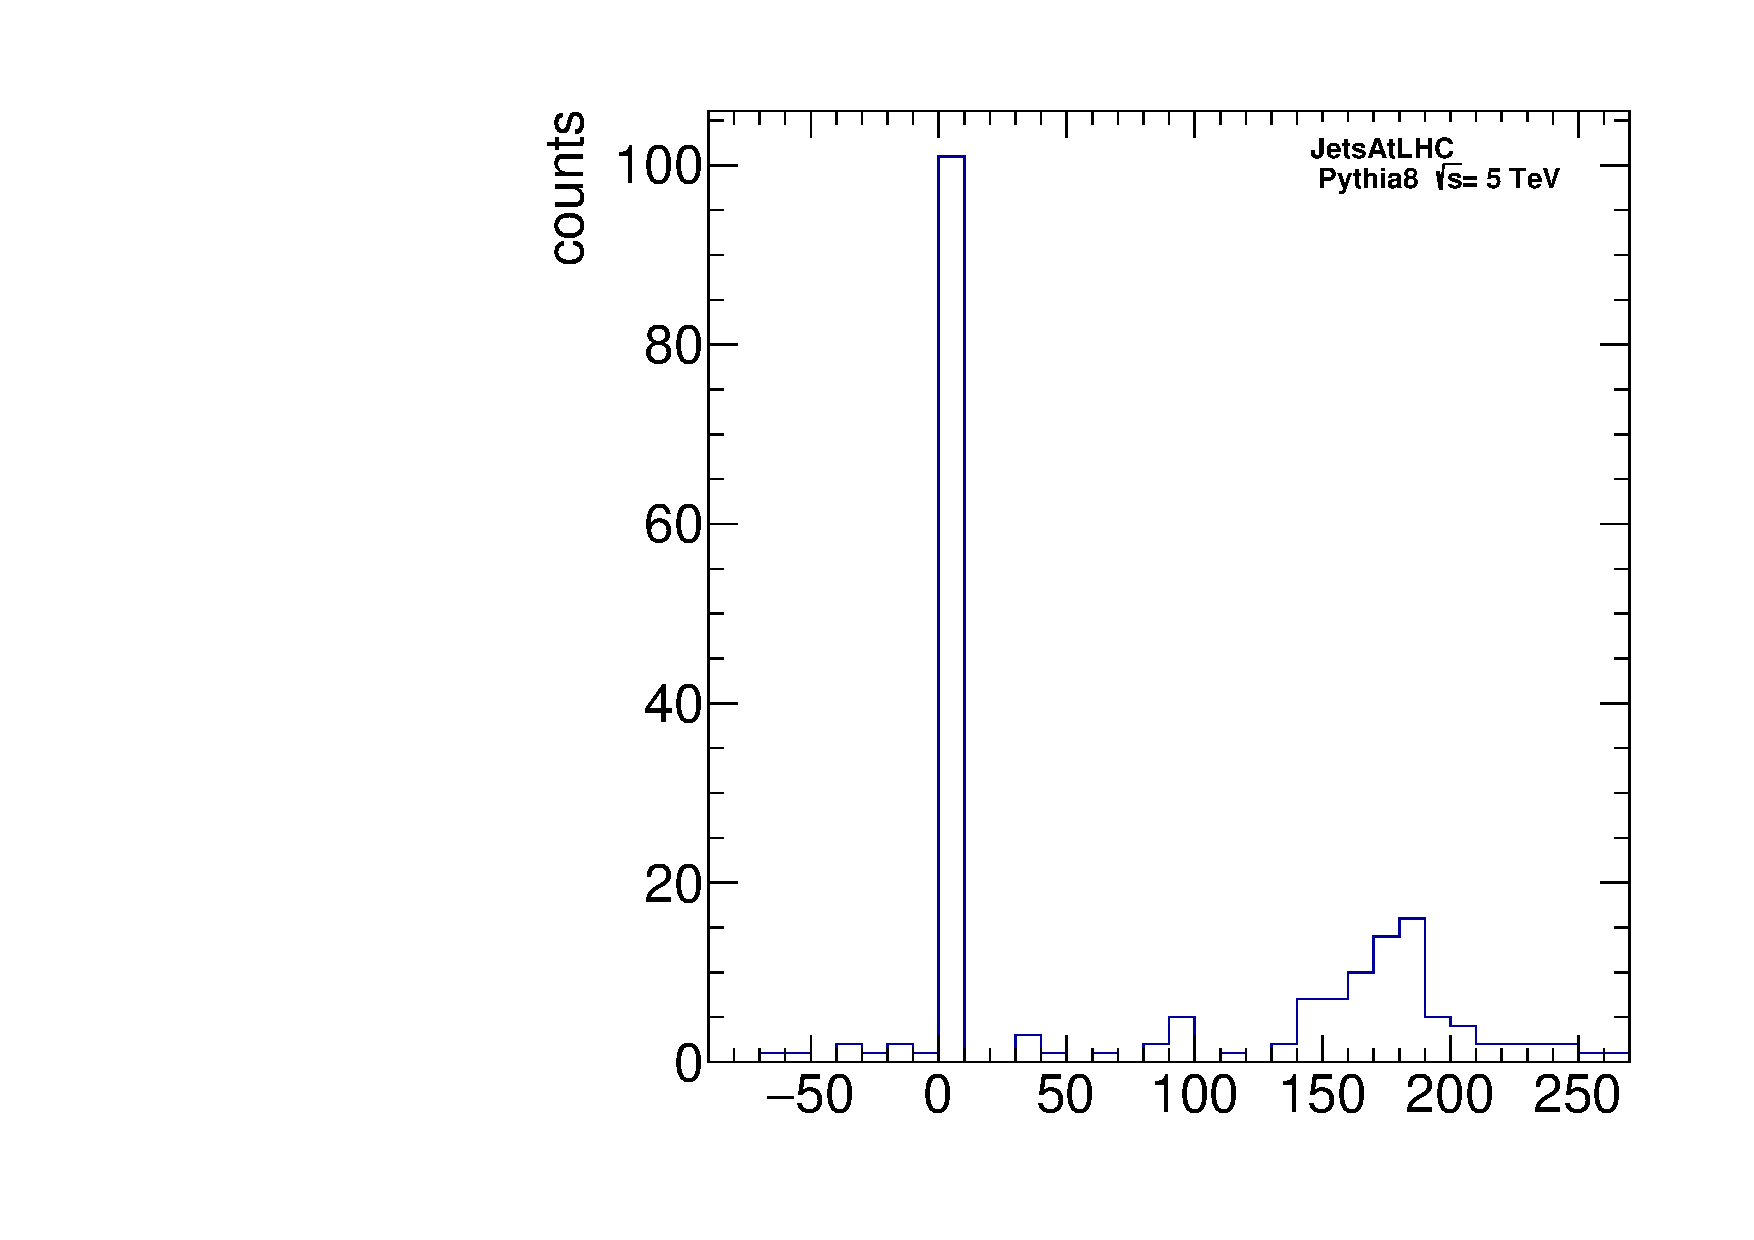
\includegraphics[width=\textwidth]{figures/hDijetPhi2.pdf}
        \caption{Histogram of azimuthal angle $\phi$ of jets. One jet in each event is set at angle $0^{\circ}$, the rest are positioned relatively to the first one. }
        \label{f7}
    \end{minipage}\hfill
    \begin{minipage}{0.33\textwidth}
    \centering
    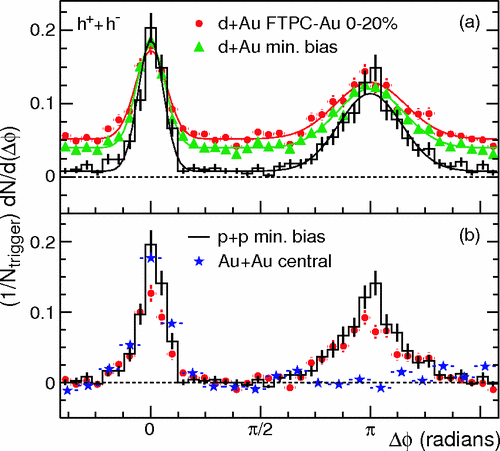
\includegraphics[width=\textwidth]{figures/jetsAtRHIC.png}
    \caption{The azimuthal angle distribution in radians measured at RHIC. Taken from Ref. \cite{jetSTAR}.}
    \label{f9}   
    \end{minipage}
    \begin{minipage}{0.33\textwidth}\hfill
        \centering
        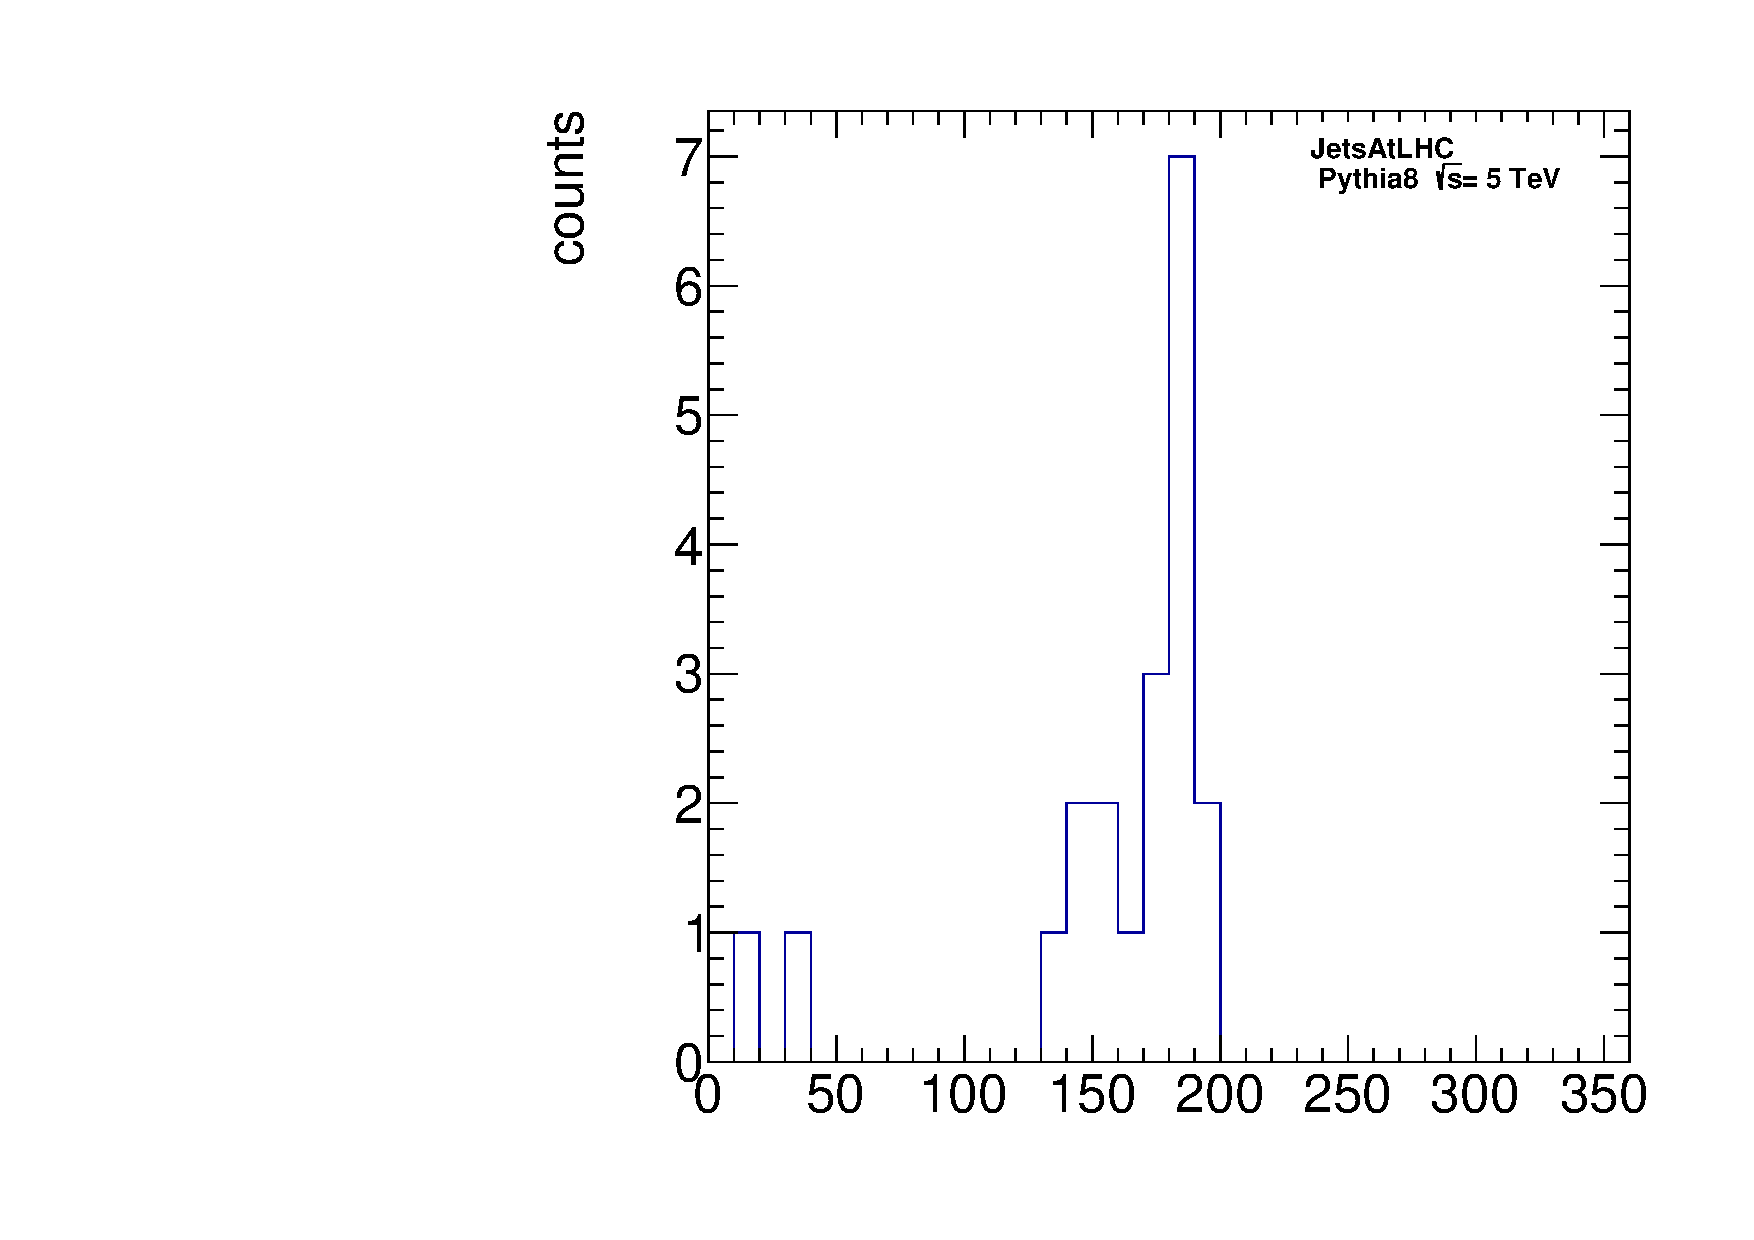
\includegraphics[width=\textwidth]{figures/hDijetPhi.pdf}
        \caption{Distribution of differences in azimuthal angle $\Delta \phi^{pairs}$ in events with exactly 2 jets.}
        \label{f8}
    \end{minipage}
\end{figure}

Next comparison to data is regarding jet imbalance. Jet imbalance is represented with variable $A_j= \frac{(p_{t,1} - p_{t,2})}{(p_{t,1} + p_{t,2})}$ and it expresses asymmetry in transverse momentum between 2 jets in a dijet. The asymmetry is more obvious in nucleus-nucleus collisions, when one of the jets loses energy by traversing the QGP medium. Otherwise from anisotropy assumption, there should not be a preferred direction of momentum. Distribution found for pairs of jets can be found in \autoref{f10}. Next to it, are distributions of the same variable for \textit{pp} and \textit{Pb-Pb} collisions with different centralities measured at the CMS detector located at the LHC. The statistics is low in \autoref{f10} therefore it does not really correspond to the shape of distribution for \textit{pp}.


\begin{figure}[htbp]
    \centering
    \begin{minipage}{0.38\textwidth}
        \centering
        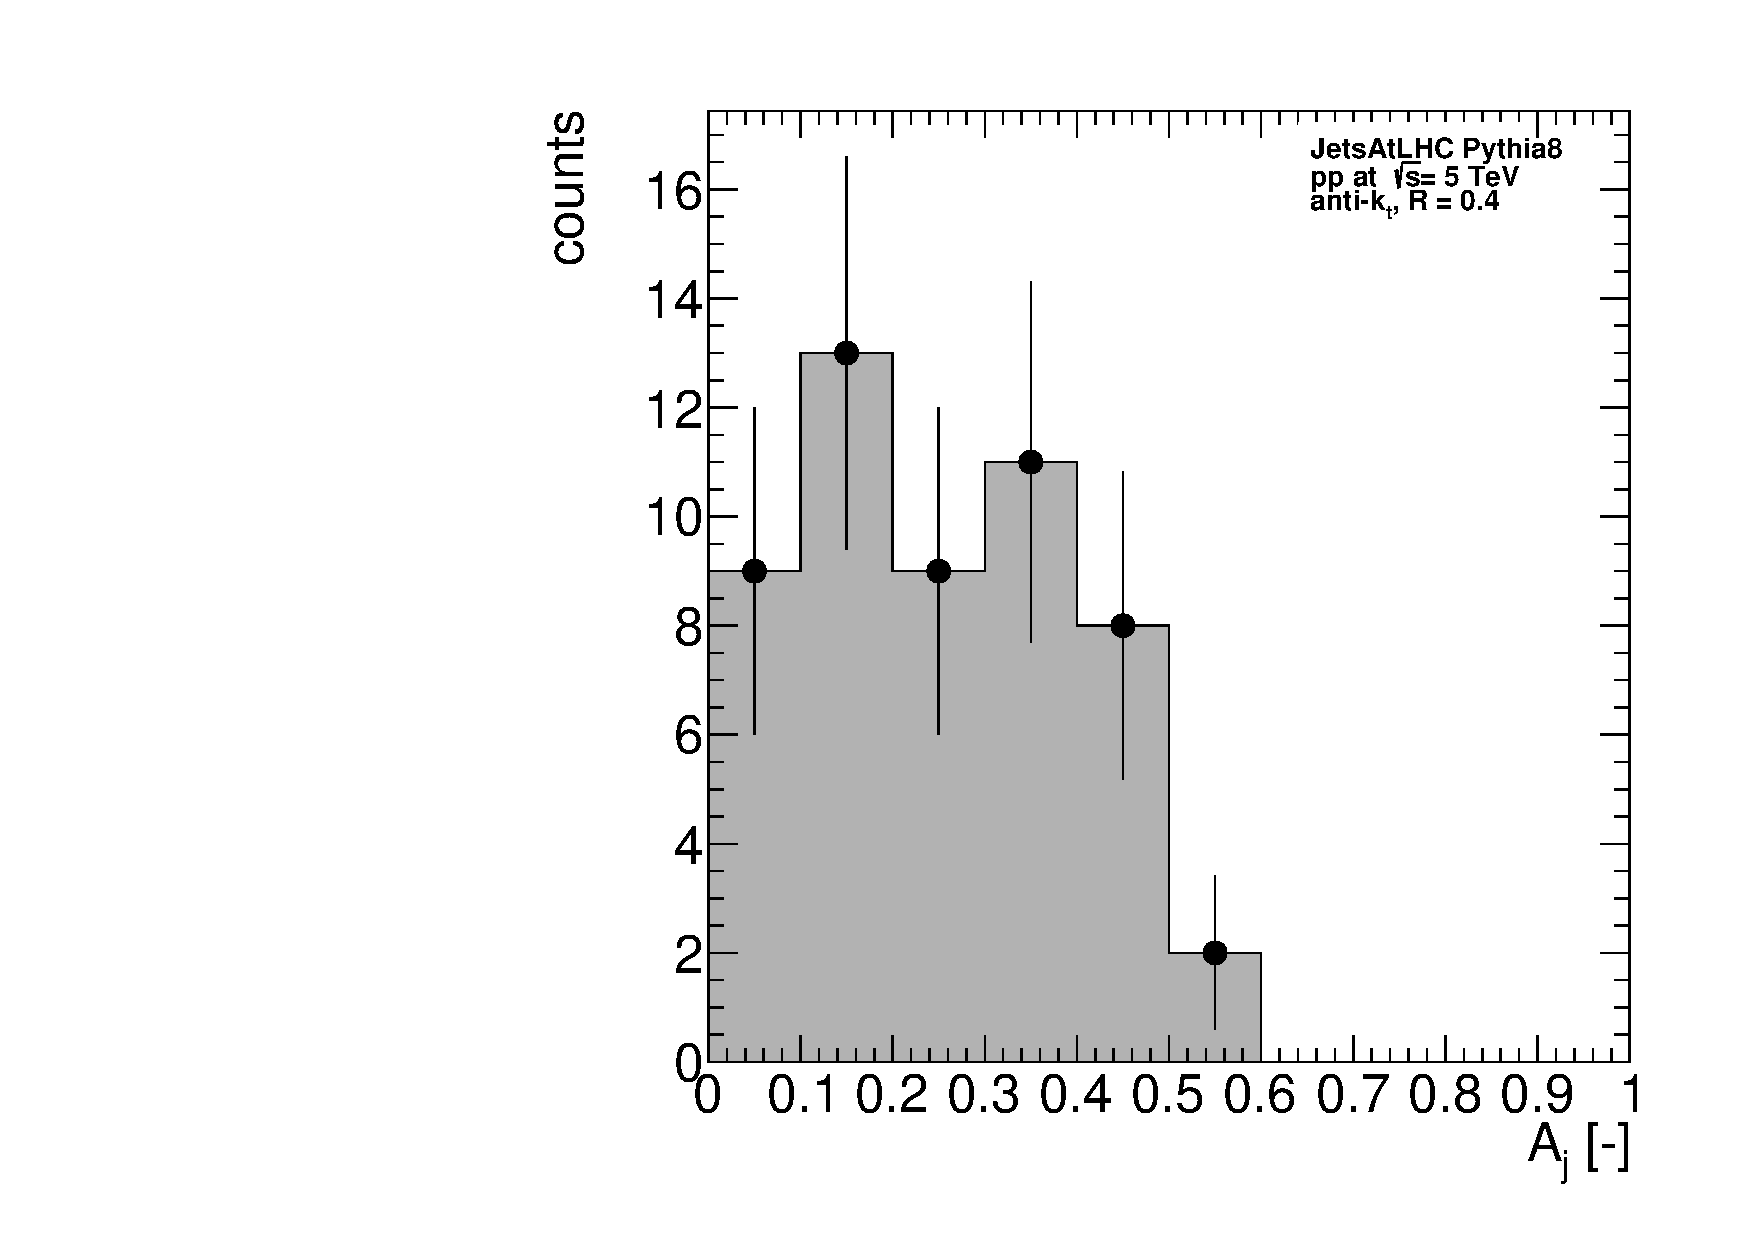
\includegraphics[width=\textwidth]{figures/hJetImbalance.pdf}
        \caption{Distribution of jet imbalance variable $A_j= \frac{(p_{t,1} - p_{t,2})}{(p_{t,1} + p_{t,2})}$ for jet pairs. }
        \label{f10}
    \end{minipage}\hfill
    \begin{minipage}{0.58\textwidth}
        \centering
        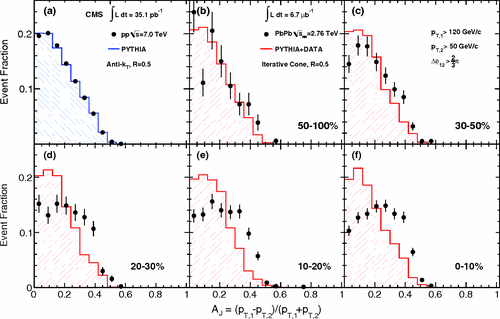
\includegraphics[width=\textwidth]{figures/pTimbalance.png}
        \caption{Distribution of variable $A_j= \frac{(p_{t,1} - p_{t,2})}{(p_{t,1} + p_{t,2})}$ for \textit{pp} collisions and heavy ion collisions with different centralities measured at the CMS detector at the LHC. Data are compared to Pythia distributions. Taken from Ref.\cite{CMS}. }
        \label{f11}
    \end{minipage}
\end{figure}

\section{CONCLUSION}
This project consisted of several parts: jets were introduced as a high energetic probes of QGP and a way to study and understand the strong force. Following, 2 softwares used in High Energy Physics: Pythia8 and FastJet3 were introduced and used to generate 100 collisions of protons at energy of collision $\sqrt{s}=5$ TeV and then used anti-$k_t$ jet algorithm to search for jets. Lastly, distributions were plotted using ROOT data analysis. The entire code can be found in Ref.\cite{GitHubJets}.
\newline
\noindent The entire project was centered around the 100 events only in proton-proton collisions. It would certainly be added value to generate more events as well as events in nucleus-nucleus collisions to compare results. The focus on results was on jet quenching and jet $p_T$ imbalance which would certainly benefit from comparison to events with QGP and to see how jets lose energy inside the QGP medium. By including more types of events, one could introduce nuclear modification factor $R_{AA}$, a variable that is specifically made for comparison between \textit{pp} and nucleus-nucleus collisions. Lastly, the analysis would benefit by including generated data from collisions with different energetic range.

\fontsize{8}{9}\selectfont

%\bibliography{ResearchPaperBib}{}
\bibliography{ResearchPaperBib}{}
%\bibliographystyle{aip}
\bibliographystyle{IEEEtran}
\addcontentsline{toc}{chapter}{Bibliography} 


\clearpage



\end{document}